
\documentclass[aspectratio=169,11pt]{beamer}

\usepackage[utf8]{inputenc}
\usepackage[T1]{fontenc}
\usepackage[spanish]{babel}

\usepackage{graphicx}
\usepackage{booktabs}
\usepackage{tabularx}
\usepackage{amsmath}

\usepackage[
    backend=biber,
    style=ieee,
    sorting=none
]{biblatex}

\addbibresource{referencias/sanchez.bib}
\addbibresource{referencias/loor.bib}
\addbibresource{referencias/zambrano.bib}

\usetheme{Madrid}
\usecolortheme{default}
\setbeamertemplate{navigation symbols}{}

\title{Computación paralela y análisis de RabbitMQ}
\subtitle{GA-SUM-02 / EXP-1}
\author{Sánchez \and Loor \and Zambrano}
\institute{Universidad Técnica Estatal de Quevedo}
\date{Noviembre de 2026}

\begin{document}

\begin{frame}
    \titlepage
\end{frame}

% Sánchez
% ============================================================
% 1. Fundamentos de la computación paralela (Sánchez)
% ============================================================
\section{Fundamentos de la computación paralela}

\begin{frame}{¿Qué es la computación paralela?}
  \begin{itemize}
    \item Divide un problema en \textbf{subtareas} que se ejecutan
          \textbf{al mismo tiempo} en varios procesadores o núcleos.
    \item Objetivo: \textbf{reducir el tiempo de cómputo} y aprovechar mejor
          los recursos.
    \item Exige \textbf{coordinación} entre quienes ejecutan las subtareas.
  \end{itemize}

  \vspace{0.3cm}
  \begin{columns}[T]
    \begin{column}{0.31\textwidth}
      \begin{block}{Memoria compartida}
        \small Núcleos de un mismo equipo comparten la memoria.
      \end{block}
    \end{column}
    \begin{column}{0.31\textwidth}
      \begin{block}{Memoria distribuida}
        \small Cada nodo tiene su memoria y se comunica por mensajes.
      \end{block}
    \end{column}
    \begin{column}{0.31\textwidth}
      \begin{block}{Híbrida}
        \small Combina ambas, como en supercomputadoras y clústeres HPC.
      \end{block}
    \end{column}
  \end{columns}

  \vspace{0.2cm}
  {\tiny Fuente: \cite{dai2025parallel}, sec.~2.1.}
\end{frame}

\begin{frame}{Paralelismo, concurrencia y sistemas distribuidos}
  \small
  \begin{tabularx}{\textwidth}{@{}p{2.6cm}XX@{}}
    \toprule
    \textbf{Concepto} & \textbf{Idea central} & \textbf{En una tienda en línea} \\
    \midrule
    Concurrencia &
      Varias tareas avanzan en un mismo período; pueden alternarse
      \cite{reinders2023}. &
      Un servidor atiende varios pedidos intercalando su ejecución. \\
    Paralelismo &
      Varias tareas se ejecutan en el mismo instante en recursos distintos
      \cite{reinders2023,dai2025parallel}. &
      Tres trabajadores procesan tres pedidos a la vez. \\
    \raggedright Sistema distribuido &
      Elementos autónomos que se comunican por red y se perciben como un
      solo sistema \cite{vansteen2023distributed}. &
      Tienda, broker y trabajadores en máquinas distintas. \\
    \bottomrule
  \end{tabularx}

  \vspace{0.3cm}
  \begin{block}{Relación}
    Se complementan: un sistema distribuido puede ejecutar en paralelo dentro
    de cada nodo; el paralelo prioriza velocidad y el distribuido,
    escalabilidad y tolerancia a fallos \cite{dai2025parallel}.
  \end{block}
\end{frame}

\begin{frame}{Ejemplo: varios trabajadores procesando pedidos}
  \begin{columns}[T]
    \begin{column}{0.47\textwidth}
      \textbf{Un trabajador (secuencial)}\\[0.15cm]
      \small
      \begin{tabular}{@{}ll@{}}
        \toprule
        Turno & Pedido \\
        \midrule
        1 a 6 & P1 $\rightarrow$ P2 $\rightarrow$ \dots $\rightarrow$ P6 \\
        \bottomrule
      \end{tabular}\\[0.15cm]
      Total: \textbf{6 turnos}.
    \end{column}
    \begin{column}{0.47\textwidth}
      \textbf{Tres trabajadores (paralelo)}\\[0.15cm]
      \small
      \begin{tabular}{@{}lll@{}}
        \toprule
        Trabajador & Turno 1 & Turno 2 \\
        \midrule
        T1 & P1 & P4 \\
        T2 & P2 & P5 \\
        T3 & P3 & P6 \\
        \bottomrule
      \end{tabular}\\[0.15cm]
      Total: \textbf{2 turnos}.
    \end{column}
  \end{columns}

  \vspace{0.3cm}
  \begin{block}{En RabbitMQ}
    Los trabajadores son consumidores de una \textbf{misma cola}: el broker
    reparte los mensajes entre ellos y entrega cada pedido a un solo
    trabajador a la vez \cite{rabbitmq2026amqp}.
  \end{block}

  {\tiny Ejemplo ilustrativo: supone pedidos independientes y de igual
  duración; no considera el costo de coordinación.}
\end{frame}

\begin{frame}{Ejemplo: pedidos de distinta duración}
  \small
  P1 y P4 tardan \textbf{4 min}; P2, P3, P5 y P6, \textbf{1 min}.
  Trabajo total: 12 min.\\[0.2cm]

  \begin{tabularx}{\textwidth}{@{}p{3.7cm}XXXc@{}}
    \toprule
    \textbf{Reparto} & \textbf{T1} & \textbf{T2} & \textbf{T3} &
      \textbf{Termina} \\
    \midrule
    \raggedright Un solo trabajador & \multicolumn{3}{l}{P1 a P6} & 12 min \\
    \raggedright Por turnos (predeterminado) & P1, P4 (8) & P2, P5 (2) &
      P3, P6 (2) & 8 min \\
    \raggedright Al quedar libre (\texttt{prefetch} = 1) & P1 (4) &
      P2, P4 (5) & P3, P5, P6 (3) & \textbf{5 min} \\
    \bottomrule
  \end{tabularx}

  \vspace{0.3cm}
  \begin{block}{Qué muestra}
    Tres trabajadores no bastan para terminar en un tercio del tiempo: importa
    cómo se reparten los pedidos. Por defecto, RabbitMQ entrega por turnos sin
    mirar cuánto trabajo tiene cada uno; con \texttt{prefetch} = 1 solo le
    entrega otro pedido a un trabajador después de su \texttt{ack}
    \cite{rabbitmq2026workqueues}.
  \end{block}

  {\tiny Ejemplo propio con duraciones supuestas; entre paréntesis, minutos
  ocupados por cada trabajador. El mínimo posible sería 4 min.}
\end{frame}

% ============================================================
% 2. Arquitectura de RabbitMQ (Sánchez)
% ============================================================
\section{Arquitectura de RabbitMQ}

\begin{frame}{RabbitMQ: qué es y qué problema resuelve}
  \begin{columns}[T]
    \begin{column}{0.44\textwidth}
      \textbf{Qué es}
      \begin{itemize}
        \item \textbf{Broker} de mensajería de código abierto
              \cite{rabbitmq2026home}.
        \item Recibe mensajes de los productores y los entrega a los
              consumidores \cite{rabbitmq2026amqp}.
        \item Implementa AMQP 0-9-1 y AMQP 1.0; también admite MQTT y
              STOMP \cite{rabbitmq2026connections}.
      \end{itemize}
    \end{column}
    \begin{column}{0.52\textwidth}
      \textbf{Qué problema resuelve en la tienda}
      \begin{itemize}
        \item \textbf{Asincronía:} la tienda registra el pedido y responde
              sin esperar a que se procese.
        \item \textbf{Desacoplamiento:} la tienda no conoce a los
              trabajadores ni al servicio de notificaciones.
        \item \textbf{Picos de carga:} si llegan muchos pedidos, esperan en
              la cola y cada trabajador toma según su capacidad.
      \end{itemize}
    \end{column}
  \end{columns}

  \vspace{0.3cm}
  {\tiny Problemas que resuelven las colas de mensajes: \cite{fu2021fair},
  sec.~I.}
\end{frame}

\begin{frame}{Usuarios, aplicaciones y escenarios de uso}
  \begin{columns}[T]
    \begin{column}{0.44\textwidth}
      \textbf{Usuarios y aplicaciones}
      \begin{itemize}
        \item Equipos que desarrollan aplicaciones web: uno de los tres
              brokers principales, junto con Kafka y Pulsar
              \cite{dyjach2024brokers}.
        \item Equipos de operación: administran colas y supervisan el
              clúster desde la interfaz web \cite{fu2021fair}.
        \item Caso real: Kodus conecta Webhooks, API y Workers con
              RabbitMQ \cite{malinosqui2026kodus}.
      \end{itemize}
    \end{column}
    \begin{column}{0.52\textwidth}
      \textbf{Escenarios de uso}\\[0.1cm]
      \small
      \begin{tabularx}{\linewidth}{@{}p{2.4cm}X@{}}
        \toprule
        Patrón & Uso \\
        \midrule
        \raggedright Cola de trabajo & Repartir los pedidos entre varios
          trabajadores. \\
        \raggedright Enrutamiento (\textit{direct}, \textit{topic}) & Enviar
          el mensaje a las colas cuya clave coincide: procesar el pedido y
          notificar al cliente. \\
        \raggedright Difusión (\textit{fanout}) & Enviar una copia a todas
          las colas vinculadas. \\
        \bottomrule
      \end{tabularx}\\[0.1cm]
      {\tiny Tipos de \textit{exchange}: \cite{rabbitmq2026amqp}.}
    \end{column}
  \end{columns}
\end{frame}

\begin{frame}{Componentes de la arquitectura}
  \small
  \begin{tabularx}{\textwidth}{@{}p{3cm}X@{}}
    \toprule
    \textbf{Componente} & \textbf{Función y ejemplo} \\
    \midrule
    Productor & Publica mensajes en un \textit{exchange}, no directamente en
      una cola. Ejemplo: la tienda
      \cite{rabbitmq2026amqp}. \\
    Conexión y canal & Conexión TCP de larga duración; los canales son
      conexiones ligeras que la comparten
      \cite{rabbitmq2026connections,rabbitmq2026channels}. \\
    \textit{Exchange} & Enruta cada mensaje a cero o más colas según su tipo
      (\textit{direct}, \textit{fanout}, \textit{topic}, \textit{headers})
      \cite{rabbitmq2026amqp}. \\
    \textit{Binding} y clave & Regla que une el \textit{exchange} con una
      cola; la clave de enrutamiento actúa como filtro
      \cite{rabbitmq2026amqp}. \\
    Cola & Guarda los mensajes en orden FIFO hasta que se consumen
      \cite{rabbitmq2026queues}. \\
    Consumidor & Recibe los mensajes, los procesa y confirma con
      \texttt{ack}. Ejemplo: los trabajadores \cite{rabbitmq2026amqp}. \\
    Broker & Servidor que recibe, enruta y entrega los mensajes; puede
      formar un clúster de varios nodos \cite{rabbitmq2026clustering}. \\
    \bottomrule
  \end{tabularx}
\end{frame}

\begin{frame}{Diagrama propio: recorrido de un pedido}
  \centering
  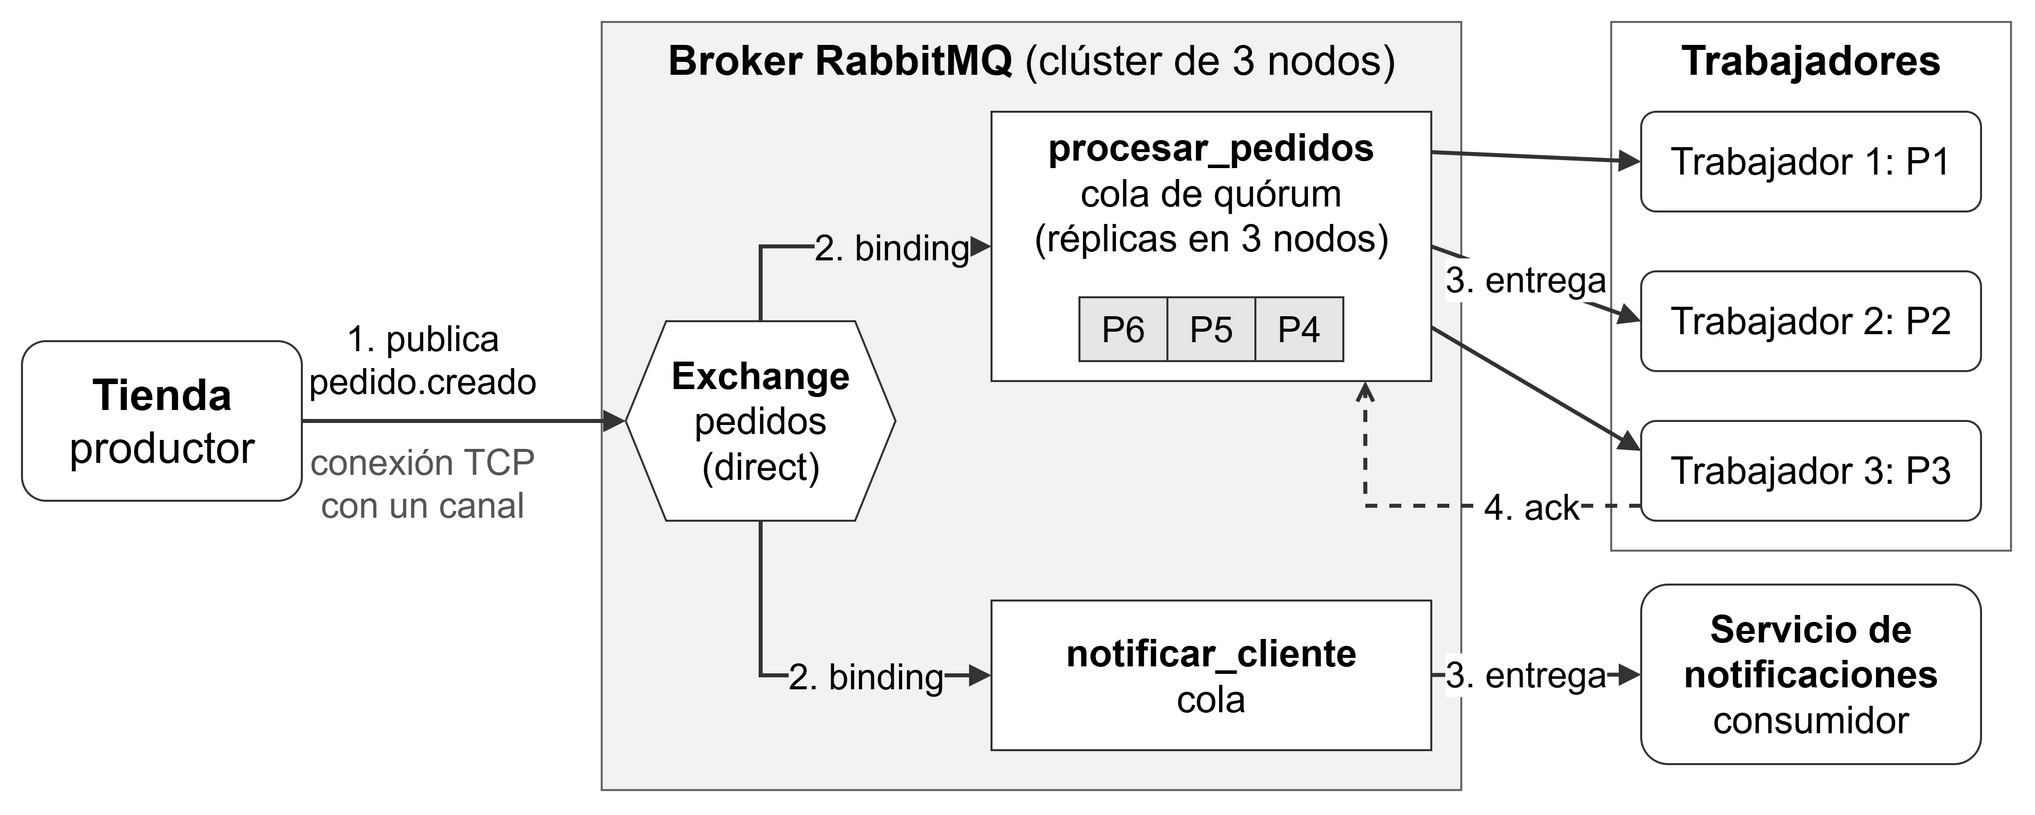
\includegraphics[width=\textwidth,height=0.68\textheight,keepaspectratio]{diagramas/arquitectura.png}

  \raggedright
  \footnotesize
  \begin{columns}[T]
    \begin{column}{0.48\textwidth}
      \begin{enumerate}
        \item La tienda publica con \texttt{pedido.creado}.
        \item El \textit{exchange} copia el pedido en ambas colas.
      \end{enumerate}
    \end{column}
    \begin{column}{0.48\textwidth}
      \begin{enumerate}
        \setcounter{enumi}{2}
        \item Cada pedido va a un solo trabajador.
        \item Sin \texttt{ack}, el pedido pasa a otro trabajador.
      \end{enumerate}
    \end{column}
  \end{columns}

  {\tiny Elaboración propia con base en
  \cite{rabbitmq2026amqp,rabbitmq2026queues,rabbitmq2026quorum}.}
\end{frame}

% ============================================================
% 3. Transparencias de distribución en RabbitMQ (Sánchez)
% ============================================================
\section{Transparencias de distribución}

\begin{frame}{Transparencias presentes en la arquitectura}
  \small
  \begin{tabularx}{\textwidth}{@{}p{2.5cm}p{3.5cm}X@{}}
    \toprule
    \textbf{Transparencia} & \textbf{Qué oculta} & \textbf{Ejemplo en el diagrama} \\
    \midrule
    Acceso & \raggedright Diferencias en cómo se representan y acceden los
      recursos. &
      La tienda y los trabajadores solo comparten el protocolo AMQP, no su
      implementación \cite{rabbitmq2026connections}. \\
    Ubicación & \raggedright Dónde está el recurso. &
      La tienda publica en el \textit{exchange} \texttt{pedidos} por su
      nombre; no sabe qué trabajador ni qué nodo atiende el pedido
      \cite{rabbitmq2026amqp,rabbitmq2026clustering}. \\
    Replicación & \raggedright Que existen varias copias. &
      \texttt{procesar\_pedidos} tiene réplicas en los 3 nodos, pero se usa
      como una sola cola \cite{rabbitmq2026quorum}. \\
    Concurrencia & \raggedright Que otros comparten el recurso. &
      Los tres trabajadores consumen de la misma cola sin coordinarse entre
      sí \cite{rabbitmq2026amqp}. \\
    Fallos & \raggedright El fallo y la recuperación. &
      Si el trabajador 3 cae sin \texttt{ack}, su pedido pasa a otro; si cae
      el nodo líder de la cola, se elige otro
      \cite{rabbitmq2026queues,rabbitmq2026quorum}. \\
    \bottomrule
  \end{tabularx}

  \vspace{0.2cm}
  {\tiny Tipos de transparencia: \cite{vansteen2023distributed}.}
\end{frame}

\begin{frame}{Limitaciones de esas transparencias}
  \begin{itemize}
    \item \textbf{Fallos:} el pedido reentregado llega marcado como
          \texttt{redelivered} y puede cambiar el orden; si el trabajador
          alcanzó a procesarlo, se procesaría dos veces
          \cite{rabbitmq2026queues,fu2021fair}.
    \item \textbf{Ubicación:} si cae el nodo al que está conectada la
          tienda, esta debe reconectarse a otro nodo
          \cite{rabbitmq2026clustering}.
    \item \textbf{Replicación:} por defecto, una cola vive en un solo nodo;
          la de quórum necesita mayoría, así que con 3 nodos tolera 1 fallo
          \cite{rabbitmq2026clustering,rabbitmq2026quorum}.
    \item \textbf{Latencia:} la tienda no sabe cuándo se procesará el
          pedido, y la demora de la red no se puede ocultar
          \cite{vansteen2023distributed}.
  \end{itemize}

  \begin{block}{Conclusión}
    La transparencia total no es alcanzable y tiene un costo en rendimiento
    \cite{vansteen2023distributed}. RabbitMQ oculta la distribución en el
    caso normal, pero ante fallos y latencia la aplicación debe intervenir.
  \end{block}
\end{frame}


% Loor

\section{CAP y PACELC en RabbitMQ}

\begin{frame}{CAP: Consistencia, Disponibilidad, Particiones}
  \small
  \begin{itemize}
    \item \textbf{Consistencia (C):} las lecturas que se realizan deben reflejar el estado más reciente de los datos.
    \item \textbf{Disponibilidad (A):} el sistema responde a cada solicitud con una respuesta válida.
    \item \textbf{Tolerancia a particiones (P):} el sistema debe afrontar interrupciones de comunicación entre sus nodos.
  \end{itemize}

  \begin{block}{¿Dónde está el problema?}
    Si los nodos dejan de comunicarse, el sistema puede tener que limitar algunas operaciones para mantener la consistencia, o seguir respondiendo con menos garantías.
  \end{block}

 \begin{block}{Ejemplo: quorum queue de RabbitMQ}
    Una cola replicada en tres miembros necesita
    una mayoría de dos para operar.

    Si uno queda aislado, la mayoría puede
    continuar; la minoría no puede confirmar
    publicaciones de forma independiente.
  \end{block}

  {\tiny Fundamento CAP: \cite{ahmed2023,myrhorodskyi2025}.
  Comportamiento de RabbitMQ: \cite{rabbitmq2026quorum}.}
\end{frame}

\begin{frame}{PACELC: consistencia frente a latencia}
  \small
  \begin{itemize}
    \item \textbf{Si hay una partición (P):} se presenta el compromiso entre la disponibilidad y la consistencia.
    \item \textbf{Si no hay una partición (E):} mantener las réplicas coordinadas solo para mantener la consistencia puede hacer que aumente la latencia.
  \end{itemize}

  \begin{block}{Aplicación a RabbitMQ}
    Las quorum queues utilizan consenso entre
    sus miembros, la necesidad de alcanzar
    una mayoría limita las operaciones cuando
    se pierde el quórum.
  \end{block}

  {\tiny Fundamento PACELC: \cite{ahmed2023,myrhorodskyi2025}.
  Caso RabbitMQ: \cite{rabbitmq2026quorum}.}
\end{frame}

\begin{frame}{Dos formas de procesar un pedido}
  \centering

  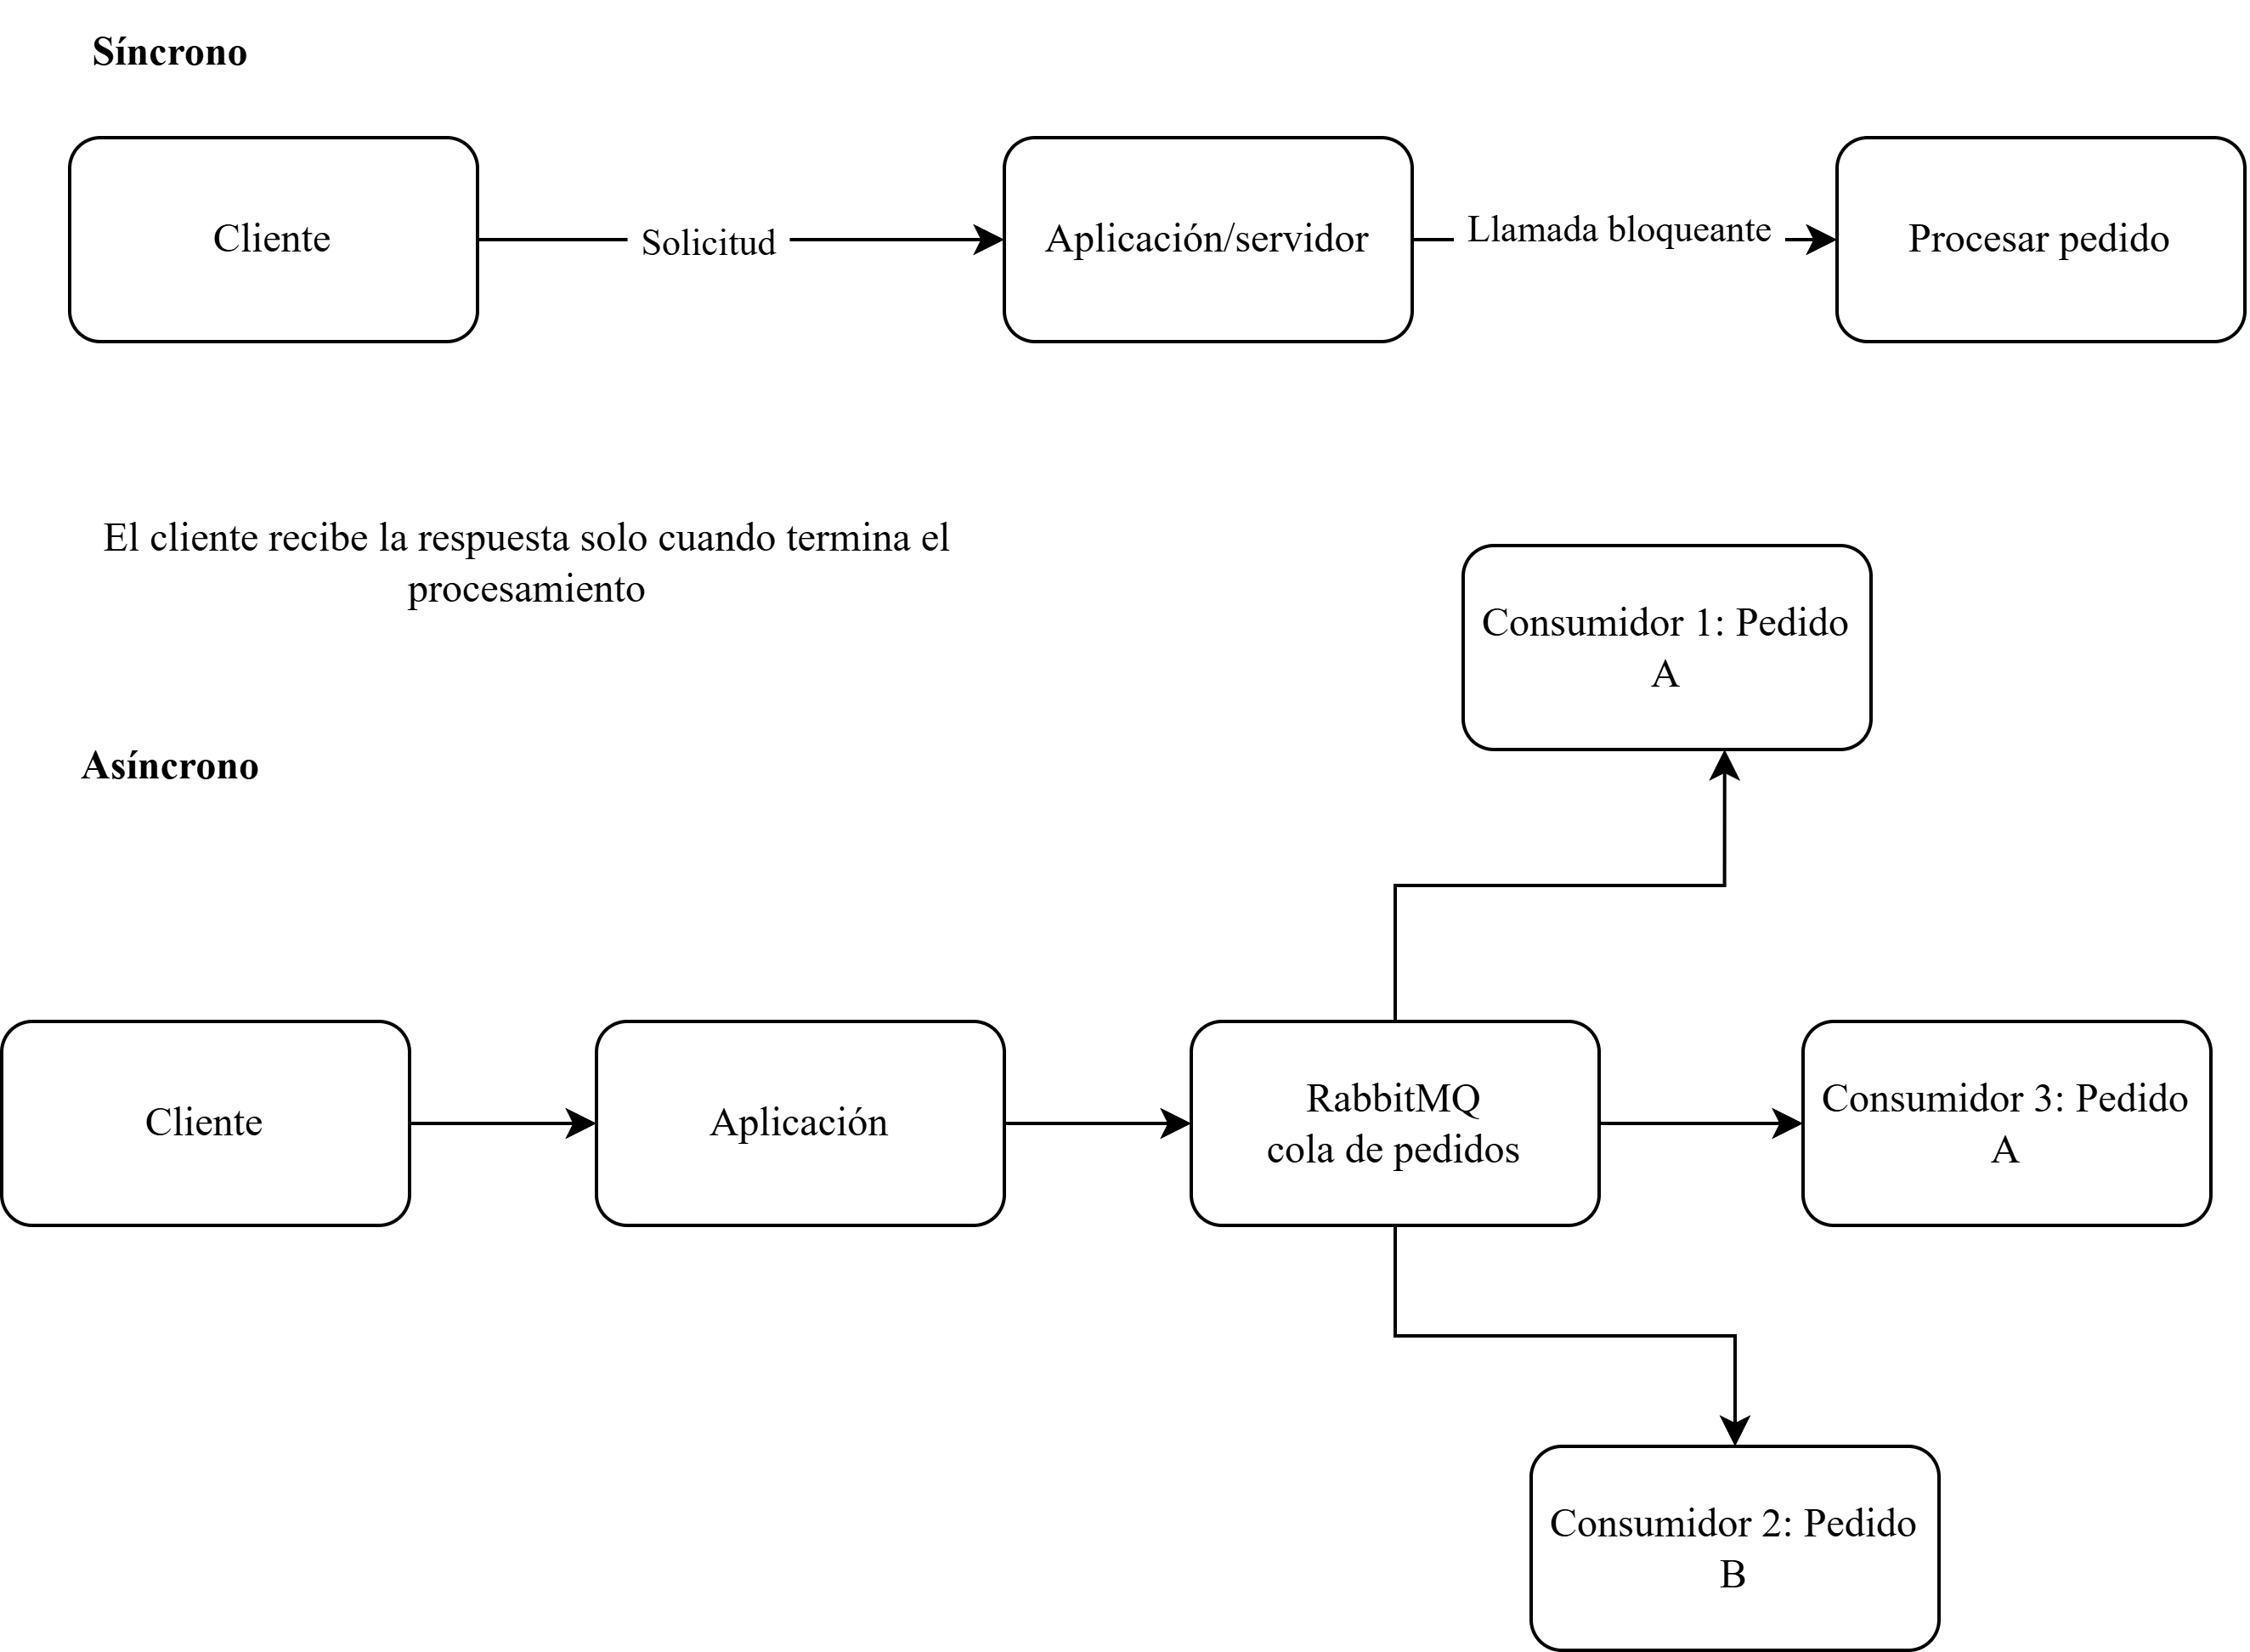
\includegraphics[
    width=0.96\textwidth,
    height=0.76\textheight,
    keepaspectratio
  ]{diagramas/procesamiento.png}

  \vspace{0.1cm}
  {\tiny Elaboración propia. Ejemplo de comunicación síncrona y asíncrona. A partir de \cite{maharjan2023,derlatka2023}. Nota: Los consumidores comparten la cola y
  procesan pedidos diferentes.}
  \end{frame}

\section{Modelos de comunicación}

\begin{frame}{Comunicación síncrona y asíncrona}
 \begin{itemize}
  \item Los procesos intercambian información
  para coordinar tareas en un sistema distribuido
  \cite{kazanavicius2023}.
  \item La comunicación puede ser
  \textbf{síncrona} o \textbf{asíncrona}
  \cite{kazanavicius2023}.
\end{itemize}

  {\tiny Fuente: \cite{kazanavicius2023}}
\end{frame}

\begin{frame}{Comunicación síncrona}
  \begin{itemize}
    \item El emisor ha realizado una solicitud y ahora está a la espera de una respuesta \cite{kazanavicius2023}.
    \item El proceso dependiente no continúa hasta que reciba el resultado.
    \item Podría provocar demoras si el receptor tarda mucho o no responde.
  \end{itemize}

  \vspace{0.3cm}
  \begin{block}{Ejemplo}
    Una tienda consulta si un pago fue aprobado y espera el resultado antes de confirmar la compra.
  \end{block}

  {\tiny Fuente: \cite{kazanavicius2023}}
\end{frame}

\begin{frame}{Comunicación asíncrona}
  \begin{itemize}
    \item El emisor envía un mensaje sin esperar el resultado de inmediato \cite{maharjan2023}.
    \item El receptor puede procesar el mensaje posteriormente.
    \item Este reduce la dependencia temporal entre los componentes \cite{kazanavicius2023}.
    \item Las colas permiten gestionar mensajes pendientes de procesamiento \cite{derlatka2023}.
  \end{itemize}

  {\tiny Fuentes: \cite{maharjan2023,derlatka2023,kazanavicius2023}}
\end{frame}

\begin{frame}{Comunicación síncrona frente a asíncrona}
  \small
  \begin{table}
    \centering
    \begin{tabularx}{\textwidth}{lXX}
      \toprule
      \textbf{Aspecto} & \textbf{Síncrona} & \textbf{Asíncrona} \\
      \midrule
      Respuesta & Espera el resultado & No espera el resultado inmediato \\
      Dependencia & Mayor dependencia temporal & Menor dependencia temporal \\
      Ventaja & Permite decidir con la respuesta & Permite continuar otras tareas \\
      Limitación & Puede generar esperas & Requiere gestionar mensajes \\
      Ejemplo & Consulta de pago & Cola de pedidos \\
      \bottomrule
    \end{tabularx}
  \end{table}

  \vspace{0.3cm}
  {\tiny Fuentes: \cite{kazanavicius2023,maharjan2023,derlatka2023}}
\end{frame}

\begin{frame}{Hilos, concurrencia y paralelismo}
  \begin{itemize}
    \item \textbf{Hilo:} es la unidad de ejecución dentro de un proceso.
    \item \textbf{Concurrencia:} dos o más hilos progresan durante un mismo período \cite{reinders2023}.
    \item \textbf{Paralelismo:} dos o más hilos se ejecutan simultáneamente \cite{reinders2023}.
  \end{itemize}

  \vspace{0.3cm}
  \begin{block}{Ejemplo}
  Tres trabajadores procesan pedidos diferentes.
  Si alternan su ejecución, existe concurrencia;
  si trabajan simultáneamente, existe paralelismo.
  \end{block}

  {\tiny Fuente: \cite{reinders2023}, cap. 1, pp. 28--29.}
\end{frame}


\begin{frame}{Modelos de comunicación}
  \begin{itemize}
    \item \textbf{Cliente-servidor:} un cliente solicita un servicio y otro proceso lo atiende \cite{zhang2023}.
    \item \textbf{Mensajería:} los procesos intercambian mensajes directamente o mediante intermediarios \cite{maharjan2023}.
    \item \textbf{RPC:} un proceso solicita la ejecución de una operación en otro proceso \cite{zhang2023}.
  \end{itemize}

  \vspace{0.3cm}
  \begin{block}{Aplicación en RabbitMQ}
    RabbitMQ actúa como intermediario entre productores y consumidores. También admite patrones de petición-respuesta \cite{maharjan2023}.
  \end{block}

  {\tiny Fuentes: \cite{zhang2023,maharjan2023}}
\end{frame}

\begin{frame}{Procesamiento asíncrono con RabbitMQ}
  \begin{enumerate}
    \item Un cliente realiza un pedido.
    \item La aplicación publica un mensaje en RabbitMQ.
    \item El broker dirige el mensaje a una cola.
    \item Un consumidor recibe y procesa el pedido.
    \item Otros consumidores pueden procesar pedidos diferentes.
  \end{enumerate}

  \vspace{0.3cm}
  \begin{block}{Ventaja}
    La aplicación puede continuar atendiendo solicitudes mientras los trabajadores procesan los pedidos.
  \end{block}

  {\tiny Fuentes: \cite{maharjan2023,kazanavicius2023,derlatka2023}}
\end{frame}

\begin{frame}{Aplicación al PFC: SREI}
\footnotesize

\begin{itemize}
    \setlength{\itemsep}{0.08cm}

    \item \textbf{Sistema:}
    Registro de Eventos Interculturales (SREI).

    \item \textbf{Servicio proveedor:}
    \texttt{servicio-eventos} (puerto 8080).
    Proporciona información de un evento intercultural.

    \item \textbf{Servicio consumidor:}
    \texttt{servicio-consulta} (puerto 8081).
    Solicita la información al proveedor y utiliza
    los datos recibidos para responder a la consulta.
\end{itemize}

\vspace{0.1cm}

\begin{block}{Implementación REST en Spring Boot}
\textbf{Proveedor (EventoController):}

\texttt{\detokenize{@GetMapping("/consulta")}}

\vspace{0.08cm}

\textbf{Consumidor (ConsultaController):}

\texttt{\detokenize{cliente.get().uri("/api/eventos/consulta")}}

\texttt{\detokenize{.retrieve().body(Map.class);}}
\end{block}

\vspace{0.1cm}

\begin{block}{Relación con la teoría}
El consumidor solicita información mediante HTTP
y espera la respuesta del proveedor para utilizarla.
Esto representa comunicación síncrona mediante REST.
\end{block}

\end{frame}

% Zambrano
% ============================================================
% 6. Fallos y tolerancia a fallos en RabbitMQ (Zambrano)
% ============================================================
\section{Fallos y tolerancia a fallos}

\begin{frame}{Riesgos de la concurrencia}
  \begin{itemize}
    \item \textbf{Condición de carrera:} dos trabajadores leen el mismo pedido y los dos lo despachan.
    \item \textbf{Bloqueo:} un trabajador espera a otro que nunca termina y la cola deja de avanzar.
    \item \textbf{Coordinación:} quién toma cada tarea y qué pasa si nadie confirma que la terminó.
  \end{itemize}
  \vspace{0.4cm}
  RabbitMQ entrega cada mensaje de una cola a un solo consumidor a la vez, pero eso no basta si el trabajador falla a mitad del proceso.
\end{frame}

\begin{frame}{Un trabajador falla con el pedido en la mano}
  \begin{enumerate}
    \item La cola entrega el pedido 125 al trabajador 1.
    \item El trabajador 1 se cae antes de terminar.
    \item Como nunca envió la confirmación (\texttt{ack}), RabbitMQ devuelve el pedido a la cola.
    \item El trabajador 2 lo recibe marcado como reentregado (\texttt{redelivered}) y lo procesa.
  \end{enumerate}
  \vspace{0.3cm}
  Si la confirmación fuera automática, el pedido se daría por entregado al salir de la cola y se perdería \cite{rabbitmq2026confirms}.
\end{frame}

\begin{frame}{Mecanismos de RabbitMQ}
  \begin{tabularx}{\textwidth}{lX}
    \toprule
    Mecanismo & Para qué sirve \\
    \midrule
    \texttt{ack} manual & El mensaje sale de la cola solo cuando el trabajador termina. \\
    \texttt{nack} / reencolar & El trabajador avisa que no pudo y el mensaje vuelve a la cola. \\
    Prefetch & Limita cuántos mensajes sin confirmar tiene cada trabajador. \\
    Publisher confirms & El broker le confirma al productor que guardó el mensaje. \\
    \bottomrule
  \end{tabularx}
  \vspace{0.3cm}
  {\small Fuente: \cite{rabbitmq2026confirms}}
\end{frame}

\begin{frame}{Incidente real: Kodus, enero de 2026}
  \begin{itemize}
    \item Migraron de un monolito a tres servicios conectados por RabbitMQ: Webhooks, API y Workers.
    \item 4 de enero: termina la migración.
    \item Días después: las revisiones de código se vuelven lentas y las máquinas se caen con carga.
    \item 23 de enero: encuentran la causa, con unos 900 \textit{pull requests} en cola.
  \end{itemize}
  \vspace{0.3cm}
  {\small Fuente: post-mortem oficial de Kodus \cite{malinosqui2026kodus}}
\end{frame}

\begin{frame}{Causas raíz del incidente de Kodus}
  \centering
  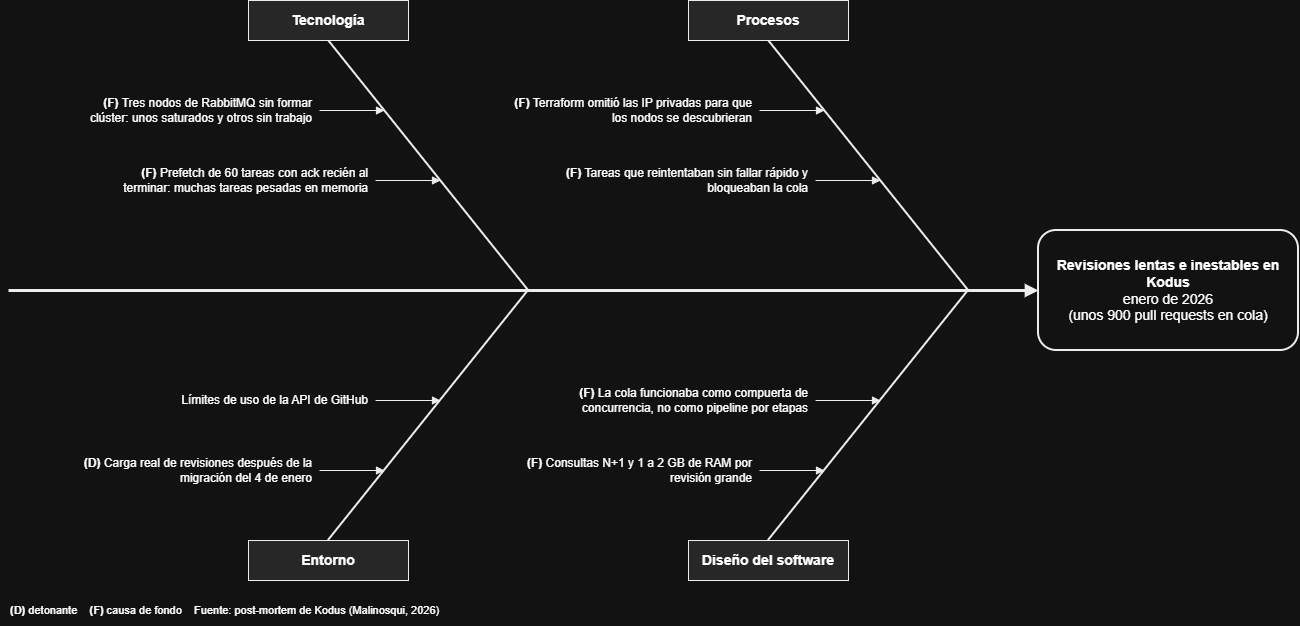
\includegraphics[width=\textwidth]{diagramas/causas.png}\\[0.2cm]
  {\small Detonante: la carga real después de la migración. Causa de fondo principal: RabbitMQ nunca funcionó como clúster \cite{malinosqui2026kodus}.}
\end{frame}

\begin{frame}{Cómo lo resolvieron}
  \begin{itemize}
    \item Corrigieron Terraform y los tres nodos formaron un solo clúster: la cola de 900 se vació en minutos.
    \item Bajaron el prefetch de 60 a 20 tareas por trabajador.
    \item Corrigieron las consultas N+1 y bajó el uso de memoria.
    \item Hicieron que las tareas trabadas pudieran salir de la cola.
  \end{itemize}
  \vspace{0.3cm}
  {\small Fuente: \cite{malinosqui2026kodus}}
\end{frame}

% ============================================================
% 7. Comparación crítica: RabbitMQ y Apache Kafka (Zambrano)
% ============================================================
\section{Comparación con Apache Kafka}

\begin{frame}{Dos formas de mover mensajes}
  \begin{columns}[T]
    \begin{column}{0.48\textwidth}
      \textbf{RabbitMQ: cola}
      \begin{itemize}
        \item El broker empuja cada mensaje a un consumidor.
        \item Cuando el trabajador confirma (\texttt{ack}), el mensaje se borra.
        \item Un pedido lo procesa un solo trabajador.
      \end{itemize}
    \end{column}
    \begin{column}{0.48\textwidth}
      \textbf{Kafka: registro (log)}
      \begin{itemize}
        \item Los mensajes se guardan en particiones, en orden.
        \item Cada consumidor lee a su ritmo y recuerda hasta dónde llegó (\textit{offset}).
        \item Los mensajes se quedan un tiempo y se pueden volver a leer.
      \end{itemize}
    \end{column}
  \end{columns}
\end{frame}

\begin{frame}{Comparación}
  \small
  \begin{tabularx}{\textwidth}{lXX}
    \toprule
    Criterio & RabbitMQ & Kafka \\
    \midrule
    Arquitectura & Exchanges que enrutan a colas & Temas divididos en particiones repartidas entre brokers \\
    Comunicación & El broker entrega (push) & El consumidor pide (pull) \\
    Procesamiento & Trabajadores que se reparten tareas & Grupos de consumidores que leen un flujo de eventos \\
    Si falla un consumidor & Lo que no confirmó vuelve a la cola & Otro consumidor sigue desde el último offset guardado \\
    Retención & Se borra al confirmar & Se guarda por tiempo o tamaño \\
    \bottomrule
  \end{tabularx}
\end{frame}

\begin{frame}{Lo que dicen las mediciones}
  \begin{itemize}
    \item Ramadan et al.: RabbitMQ tuvo menor latencia por mensaje en casi todos los escenarios; con mensajes de 100 KB, unos 4,38 ms frente a 83,27 ms de Kafka. Kafka fue más estable con carga extrema y sostenida \cite{rias2026kafka}.
    \item Kamiński et al.: el resultado depende del entorno. En .NET, Kafka logró hasta 38\,\% más rendimiento y 40\,\% menos latencia; en Spring Boot, RabbitMQ usó 29\,\% menos memoria y respondió 25\,\% más rápido \cite{kaminski2025rabbitmq}.
  \end{itemize}
  \vspace{0.3cm}
  Ninguno gana siempre: depende de la carga y de la plataforma.
\end{frame}

\begin{frame}{Cuándo conviene cada uno}
  \begin{tabularx}{\textwidth}{XX}
    \toprule
    RabbitMQ & Kafka \\
    \midrule
    Pedidos o tareas que un trabajador procesa una sola vez y confirma & Flujos de eventos que varios sistemas leen por separado \\
    Notificaciones y correos & Auditoría y analítica, donde hace falta volver a leer el historial \\
    Enrutamiento flexible entre colas & Volúmenes muy grandes y sostenidos \\
    \bottomrule
  \end{tabularx}
  \vspace{0.3cm}
  {\small En Kodus el problema no fue elegir RabbitMQ, sino configurarlo mal: el clúster nunca se formó \cite{malinosqui2026kodus}.}
\end{frame}

% ============================================================
% 8. Conclusiones (Zambrano)
% ============================================================
\section{Conclusiones}

\begin{frame}{Lo que le sirve del caso Kodus al SGIRI}
  \begin{itemize}
    \item Revisar que el clúster de RabbitMQ se forme de verdad (\texttt{rabbitmqctl cluster\_status}), no darlo por hecho.
    \item Prefetch alto con \texttt{ack} al final llena la memoria del trabajador.
    \item Los reintentos necesitan una salida, si no un aviso trabado frena la cola de todos.
    \item Agregar trabajadores no arregla un error de configuración.
    \item El monitoreo se monta antes de migrar, no después \cite{malinosqui2026kodus}.
  \end{itemize}
\end{frame}

\begin{frame}{Si el SGIRI usara RabbitMQ para los avisos}
  \begin{tabularx}{\textwidth}{lX}
    \toprule
    Qué configurar & Para qué \\
    \midrule
    Cola \textit{quorum} durable & El aviso queda replicado y en disco \\
    \textit{Publisher confirms} & El sistema sabe que el broker recibió el aviso \\
    \texttt{ack} manual & Se confirma solo después de enviar la notificación \\
    Cola de mensajes muertos & Tras 3 intentos fallidos el aviso sale de la cola y no se pierde \\
    Prefetch bajo (5 a 10) & Cada notificación es corta, no hace falta acumular \\
    Patrón \textit{outbox} & Incidencia y aviso se guardan juntos en PostgreSQL \\
    \bottomrule
  \end{tabularx}
  \vspace{0.2cm}
  {\small Confirmaciones: \cite{rabbitmq2026confirms}}
\end{frame}

\begin{frame}{Conclusión: RabbitMQ o Kafka}
  \begin{itemize}
    \item RabbitMQ cuando cada mensaje es una tarea que se procesa, se confirma y se borra. Es el caso del SGIRI: incidencias, asignación de técnicos y avisos.
    \item Kafka cuando hay un flujo grande y continuo de eventos que varios consumidores leen a su ritmo y que hay que guardar, por ejemplo la telemetría de los equipos de red.
    \item Las mediciones no dan un ganador fijo, depende de la carga y la plataforma \cite{rias2026kafka,kaminski2025rabbitmq}.
  \end{itemize}
  \vspace{0.3cm}
  Para el SGIRI elegiría RabbitMQ, bien configurado y monitoreado.
\end{frame}


% Referencias
\begin{frame}[allowframebreaks]{Referencias}
    \printbibliography[heading=none]
\end{frame}

\end{document}
